\documentclass{standalone}
\usepackage{tikz}
\usepackage{pgf}
\usetikzlibrary{graphs}
\usetikzlibrary{shapes}
% \usegdlibrary{layered}

\pgfdeclareradialshading{ballshading}{\pgfpoint{-12bp}{10bp}}
{color(0bp)=(red!15!white);
color(5bp)=(red!15!white);
color(6bp)=(red);
% color(18bp)=(red!70!black);
% color(25bp)=(red!50!black);
color(50bp)=(red)
}

\pgfdeclareradialshading{ballshading1}{\pgfpoint{-12bp}{10bp}}
{color(0bp)=(orange!15!white);
color(5bp)=(orange!15!white);
color(6bp)=(orange);
% color(18bp)=(orange!70!black);
% color(25bp)=(orange!50!black);
color(50bp)=(orange)
}


% \tikzstyle{type0} = [circle, shading=ball, ball color=yellow, draw=yellow!50!red, thick, label=0]
\tikzstyle{type0} = [shading=ballshading,fill=green!10!yellow, draw=yellow!50!red, thick, label=0]
\tikzstyle{type1} = [shading=ballshading1,circle, fill=yellow!10!red, draw=yellow!90!red, thick, label=1]
\tikzstyle{type2} = [circle, fill=white!90!red, draw=yellow!50!red, thick, label=2]
\begin{document}
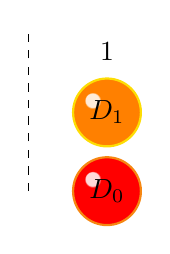
\begin{tikzpicture}[fill=red, every node/.style={draw, circle, thick, radius=3pt}, centered]
  % \node (0-1) at (10,0) {hey};
  % \foreach \x [count = \i] in {2,...,5}
    % \node (0-\x) [left of=0-\i] {\x};
  %\graph [grow right, branch down]
  %{root -> {
  %  a [type0] -> b[type2],
  %  c -> d,
  %  e -> f
  %}};

  \node (d0) [type0] at (11,0) {$D_0$};
  %\node (d0) [fill=red] at (11,0) {$D_0$};
  %\node [fill=white!80!red, x radius=1pt, y radius=2pt, shift={(-3pt,1pt)}] at (11,0) {};
  \node (d1) [type1, above of=d0] {$D_1$};
  %\node (d2) [above of=d1] {$D_2$};
  %\node (d3) [above of=d2] {$D_3$};
  % \filldraw (11,0) circle [line width=1pt,radius=1, fill=red];
  % \filldraw (11,0) circle [fill=white!80!red, x radius=0.2, y radius=0.3,rotate=-35, shift={(-0.6,0)}];
  % \filldraw (4,0) circle (.5cm) (4.5,0) circle (.5cm);
  \path (10,0) edge [draw, dashed] (10, 2);



  

\end{tikzpicture}

\end{document}
